% You should title the file with a .tex extension (hw1.tex, for example)
\documentclass[11pt]{article}

\usepackage{amsmath}
\usepackage{amssymb}
\usepackage{fancyhdr}
\usepackage{listings}
\usepackage{color}
\usepackage{graphicx}
\graphicspath{ {images/} }
\usepackage{hyperref}
\usepackage{mathtools}

\definecolor{dkgreen}{rgb}{0,0.6,0}
\definecolor{gray}{rgb}{0.5,0.5,0.5}
\definecolor{mauve}{rgb}{0.58,0,0.82}

\lstset{frame=tb,
  language=Java,
  aboveskip=3mm,
  belowskip=3mm,
  showstringspaces=false,
  columns=flexible,
  basicstyle={\small\ttfamily},
  numbers=none,
  numberstyle=\tiny\color{gray},
  keywordstyle=\color{blue},
  commentstyle=\color{dkgreen},
  stringstyle=\color{mauve},
  breaklines=true,
  breakatwhitespace=true,
  tabsize=3
}

\oddsidemargin0cm
\topmargin-2cm     %I recommend adding these three lines to increase the 
\textwidth16.5cm   %amount of usable space on the page (and save trees)
\textheight23.5cm  

\newcommand{\question}[2] {\vspace{.25in} \hrule\vspace{0.5em}
\noindent{\bf #1: #2} \vspace{0.5em}
\hrule \vspace{.10in}}
\renewcommand{\part}[1] {\vspace{.10in} {\bf (#1)}}

\newcommand{\myname}{Chang-Hyun Mungai}
\newcommand{\myhwnum}{BST Notes}

\setlength{\parindent}{0pt}
\setlength{\parskip}{5pt plus 1pt}
 
\pagestyle{fancyplain}
\lhead{\fancyplain{}{\textbf{\myhwnum}}}      % Note the different brackets!

\begin{document}

\medskip                        % Skip a "medium" amount of space
                                % (latex determines what medium is)
                                % Also try: \bigskip, \littleskip

\thispagestyle{plain}
\begin{center}                  % Center the following lines
{\Large Common Binary Search Trees} \\
\end{center}

\question{Big O}

\begin{itemize}
  \item space O(n)
  \item time
\begin{itemize}
  \item search worst O(n), average O(log(n))
  \item insert worst O(n), average O(log(n))
  \item delete worst O(n), average O(log(n))
\end{itemize}
\end{itemize}

\question{BST Node}

\begin{itemize}
  \item Data
  \item Left Child
  \item Right Child
\end{itemize}

\question{Comparison}

\begin{itemize}
  \item advantages
\begin{itemize}
  \item related sorting algorithms
  \item search algorithms
  \item inorder traversal
\end{itemize}
  \item disadvantages
\begin{itemize}
  \item shape depends on insertions
  \item keys has to be compared when inserting or searching
  \item height grows (todo: square root) n, which grows much faster than log n
\end{itemize}

  \item uses
\begin{itemize}
  \item sets, multisets, associative arrays, priority queue
\end{itemize}
\end{itemize}

\question{Operations}

\begin{itemize}
  \item Look-Up
	\begin{itemize}
 	 \item compare to current node: go left if less, go right if greater
	\end{itemize}
  \item Insert
	\begin{itemize}
 	 \item Same as look-up but replace node where it should be
	\end{itemize}
  \item Delete
	\begin{itemize}
 	 \item no children: just delete
 	 \item 1 child: remove node and replace it with the child
 	 \item 2 children: find in-order successor or predecessor R to the current node N, switch it with N then call delete on the respective child with N)
	\end{itemize}
\end{itemize}

\question{Traversals}

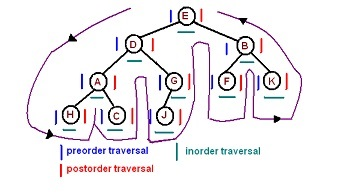
\includegraphics{traversal}

\begin{itemize}
  \item In-Order
	\begin{itemize}
 	 \item Traverse left node, current node, then right
 	 \item everything in order
	\end{itemize}
  \item Pre-Order
	\begin{itemize}
 	 \item Traverse current node, left node, then right
 	 \item while duplicating nodes and edges can make duplicate binary tree
	\end{itemize}
  \item Post-Order
	\begin{itemize}
 	 \item Traverse left node, right node, then current
 	 \item while deleting and freeing can delete and free an entire tree
	\end{itemize}
\end{itemize}

\question{AVL}

\begin{itemize}
  \item General
\begin{itemize}
      \item rebalance when insertion so that height never exceeds O(log n)
      \item shape of tree changes during insertion and deletion
      \item the height of an AVL tree is at most ~1.44log(N)
      \item AVL tree may need O(log(N)) operations to rebalance the tree
\end{itemize}
  \item searching-BST
  \item insertion - check balance factor for all ancestors if $\mid$ balance factor $\mid$ $\textgreater$ 1 then rebalance
\begin{itemize}
      \item balance factor = height(left sub tree) - height(right sub tree)
      \item rebalance starts from the inserted node up (from bottom up)
\end{itemize}
  \item deletion
\begin{itemize}
      \item Let node X be the node with the value we need to delete, and let node Y be a node in the tree we need to find to take node X's place, and let node Z be the actual node we take out of the tree
      \item Steps to consider when deleting a node in an AVL tree are the following:
\begin{itemize}
         \item If node X is a leaf or has only one child, skip to step 5 with Z:=X.
         \item Otherwise, determine node Y by finding the largest[citation needed] node in node X's left subtree (the in -order predecessor of X (todo: then) it does not have a right child) or the smallest in its right subtree (the in-order successor of X (todo: then) it does not have a left child).
         \item Exchange all the child and parent links of node X with those of node Y. In this step, the in      \item order sequence between nodes X and Y is temporarily disturbed, but the tree structure doesn't change.
         \item Choose node Z to be all the child and parent links of old node Y = those of new node X.
         \item If node Z has a subtree (which then is a leaf), attach it to Z's parent.
         \item If node Z was the root (its parent is null), update root.
         \item Delete node Z.
         \item Retrace the path back up the tree (starting with node Z's parent) to the root, adjusting the balance factors as needed.
\end{itemize}
\end{itemize}
\end{itemize}

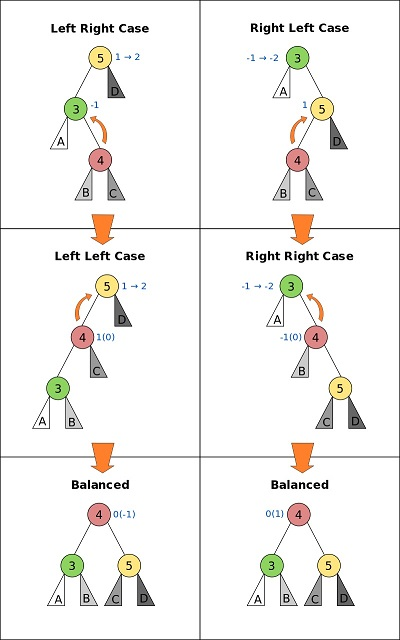
\includegraphics{AVL_Tree_Rebalancing}

\question{Red/Black}

\begin{itemize}
  \item General
\begin{itemize}
      \item the maximum height of a red-black tree, $\sim$ 2log(N)
      \item red-black tree needs O(1) operations to rebalance the tree
      \item each node has an extra bit for color red or black
\end{itemize}
  \item In addition to the requirements imposed on a binary search tree the following must be satisfied by a red–black tree
\begin{itemize}
      \item A node is either red or black
      \item The root is black. This rule is sometimes omitted. Since the root can always be changed from red to black, but not necessarily vice versa, this rule has little effect on analysis
      \item All leaves (NIL) are black
      \item If a node is red, then both its children are black
      \item Every path from a given node to any of its descendant NIL nodes contains the same number of black nodes. The uniform number of black nodes in the paths from root to leaves is called the black height of the red–black tree
\end{itemize}
  \item searching-BST
  \item insertion O(log n)
\begin{itemize}
      \item Insert as BST
      \item Fix any red-black vialations starting with inserted node continuing up the path
\end{itemize}
  \item deletion O(log n)
\begin{itemize}
      \item Delete as BST
      \item Restore red-black properties
\end{itemize}
\end{itemize}

\question{Splay}

\begin{itemize}
  \item General
\begin{itemize}
      \item rebalance when look-up so frequently accessed elements move up
      \item rebalances on look-up
      \item shapes is not constrained and depends on look-ups
\end{itemize}
  \item Advantages
\begin{itemize}
      \item ave case is efficient as others
      \item small memory
      \item works with duplicate keys
\end{itemize}
  \item Disadvantages-height can be linear
  \item splaying - x=accessed node, p=parent of x, g parent of p
\begin{itemize}
      \item when p is the root tree is rotated on edge between p and x
      \item 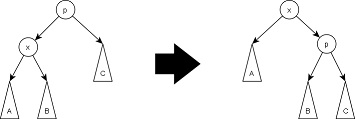
\includegraphics{splayzig}
      \item p is not the root and x and p are either both right children or are both left children
      \item 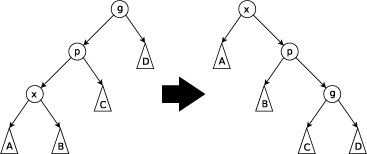
\includegraphics{splayzigzig}
      \item p is not the root and x is a right child and p is a left child or vice versa
      \item 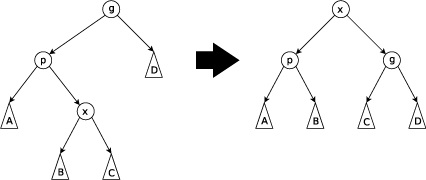
\includegraphics{splayzigzag}
\end{itemize}
\end{itemize}

\question{Comparisons}

\begin{itemize}
\item AVL trees
\begin{itemize}
\item AVL trees gurantee fast lookup (O(log n)) on each operation
\item AVL more useful in multithreaded environ with lots of look-ups because can be done in parallel (splay not in parallel)
\item Real time (and more) look-ups AVL is better
\end{itemize}
\item Red Black
\begin{itemize}
\item red black better with more inserts and deletes
\end{itemize}
\item Splay trees
\begin{itemize}
\item Splay trees gurantee any sequence of n operations take at most O(nlog n)
\item Splay faster on average on more look-ups
\item Splay better for splitting and merging efficiently
\item Splay more memory efficient (no need to store balance info)
\item Splay more effective when you only access a small subset
\item Splay rotation logic easier therefore easier to implement
\end{itemize}
\end{itemize}

\question{Notes}

\begin{itemize}
  \item Not all binary trees are BST
  \item Balancing
  \item Height: longest path from root to leaf
  \item Depth: The depth of a node is the number of edges from the node to the tree's root node
\end{itemize}

\question{sources}

\begin{itemize}
\item \url{https://en.wikipedia.org/wiki/AVL_tree}
\item \url{https://en.wikipedia.org/wiki/Red%E2%80%93black_tree}
\item \url{https://www.cs.usfca.edu/~galles/visualization/RedBlack.html}
\item \url{https://www.topcoder.com/community/data-science/data-science-tutorials/an-introduction-to-binary-search-and-red-black-trees/}
\item \url{https://en.wikipedia.org/wiki/Splay_tree}
\item \url{https://attractivechaos.wordpress.com/2008/10/02/comparison-of-binary-search-trees/}
\end{itemize}

\end{document}

